\section{ESMF Classes}

We divide the ESMF classes into three main categories: those associated 
with the coupling superstructure, those associated with the data handling
infrastrucure, and those that are part of the utility layer.  
Superstructure and Infrastructure
classes are based on a hierarchical 
calling tree of increasingly abstract data structures that represent the field data associated 
with the physical systems being modeled.  
Superstructure classes provide methods which invoke user-supplied code;
Infrastructure classes provide methods which are invoked by
user-supplied code.
Utility classes are independent 
of the data classes, though they too have a hierarchical structure; 
higher-level utilities employ general-purpose tools such as a message log.

In the listing of classes below we provide a description of each class and its function.

\subsection{ESMF Base Object}

All objects above are based on the object below.  Attributes
can be handled by generic routines, but it is expected that 
higher level objects will supply their own class specific
methods of the ones listed below.

\scalebox{0.70}{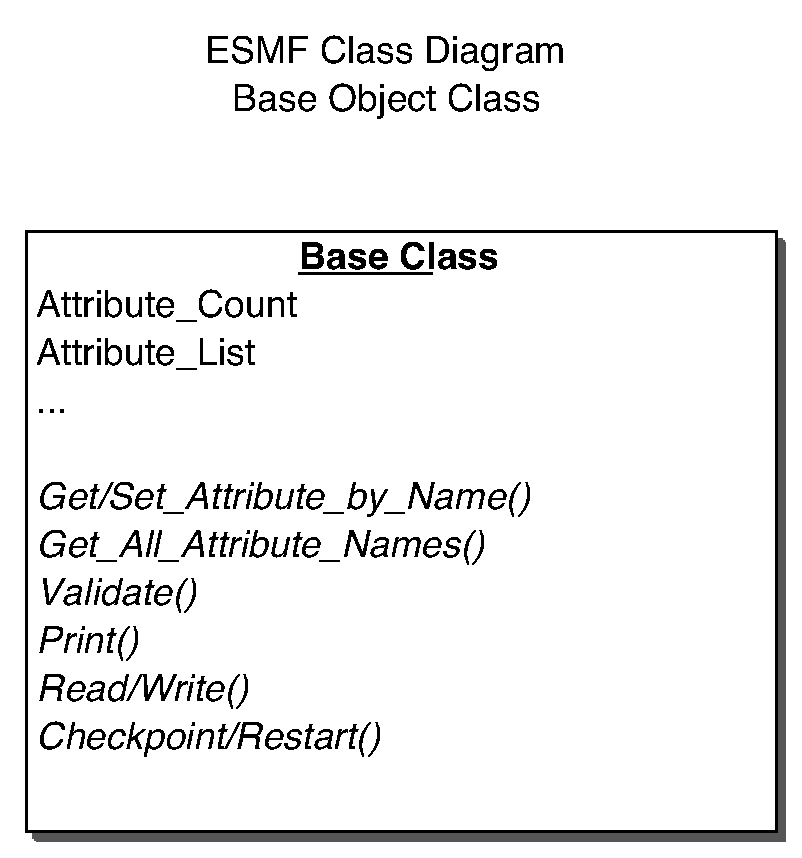
\includegraphics{ESMF_Base}}

\subsubsection{Base (ESMF\_Base)}
\label{sec:Base} 
\begin{description}
\item [Description] The ESMF Base class is an abstraction of the private data and
methods common to all other object in the system.  Some methods and data can be
inherited direcly from the Base class; others are expected to be overloaded by
higher level objects.
\item [Function] The Base class methods which are expected to be overloaded by
more specialized objects include: Print, Validate, Read/Write, Checkpoint/Restart.
Methods which are inherited by all other classes include those which 
set and query object Attributes.
\end{description}

<< perhaps the usage section goes here, or perhaps this doesn't
belong here and does belong combined with the usage section >>







